% =============================================
% 导言区
% =============================================
\documentclass{xjtureport}








% =============================================
% 正文区
% =============================================


\begin{document}

% ===导入实验报告封面==============================
\begin{titlepage}
	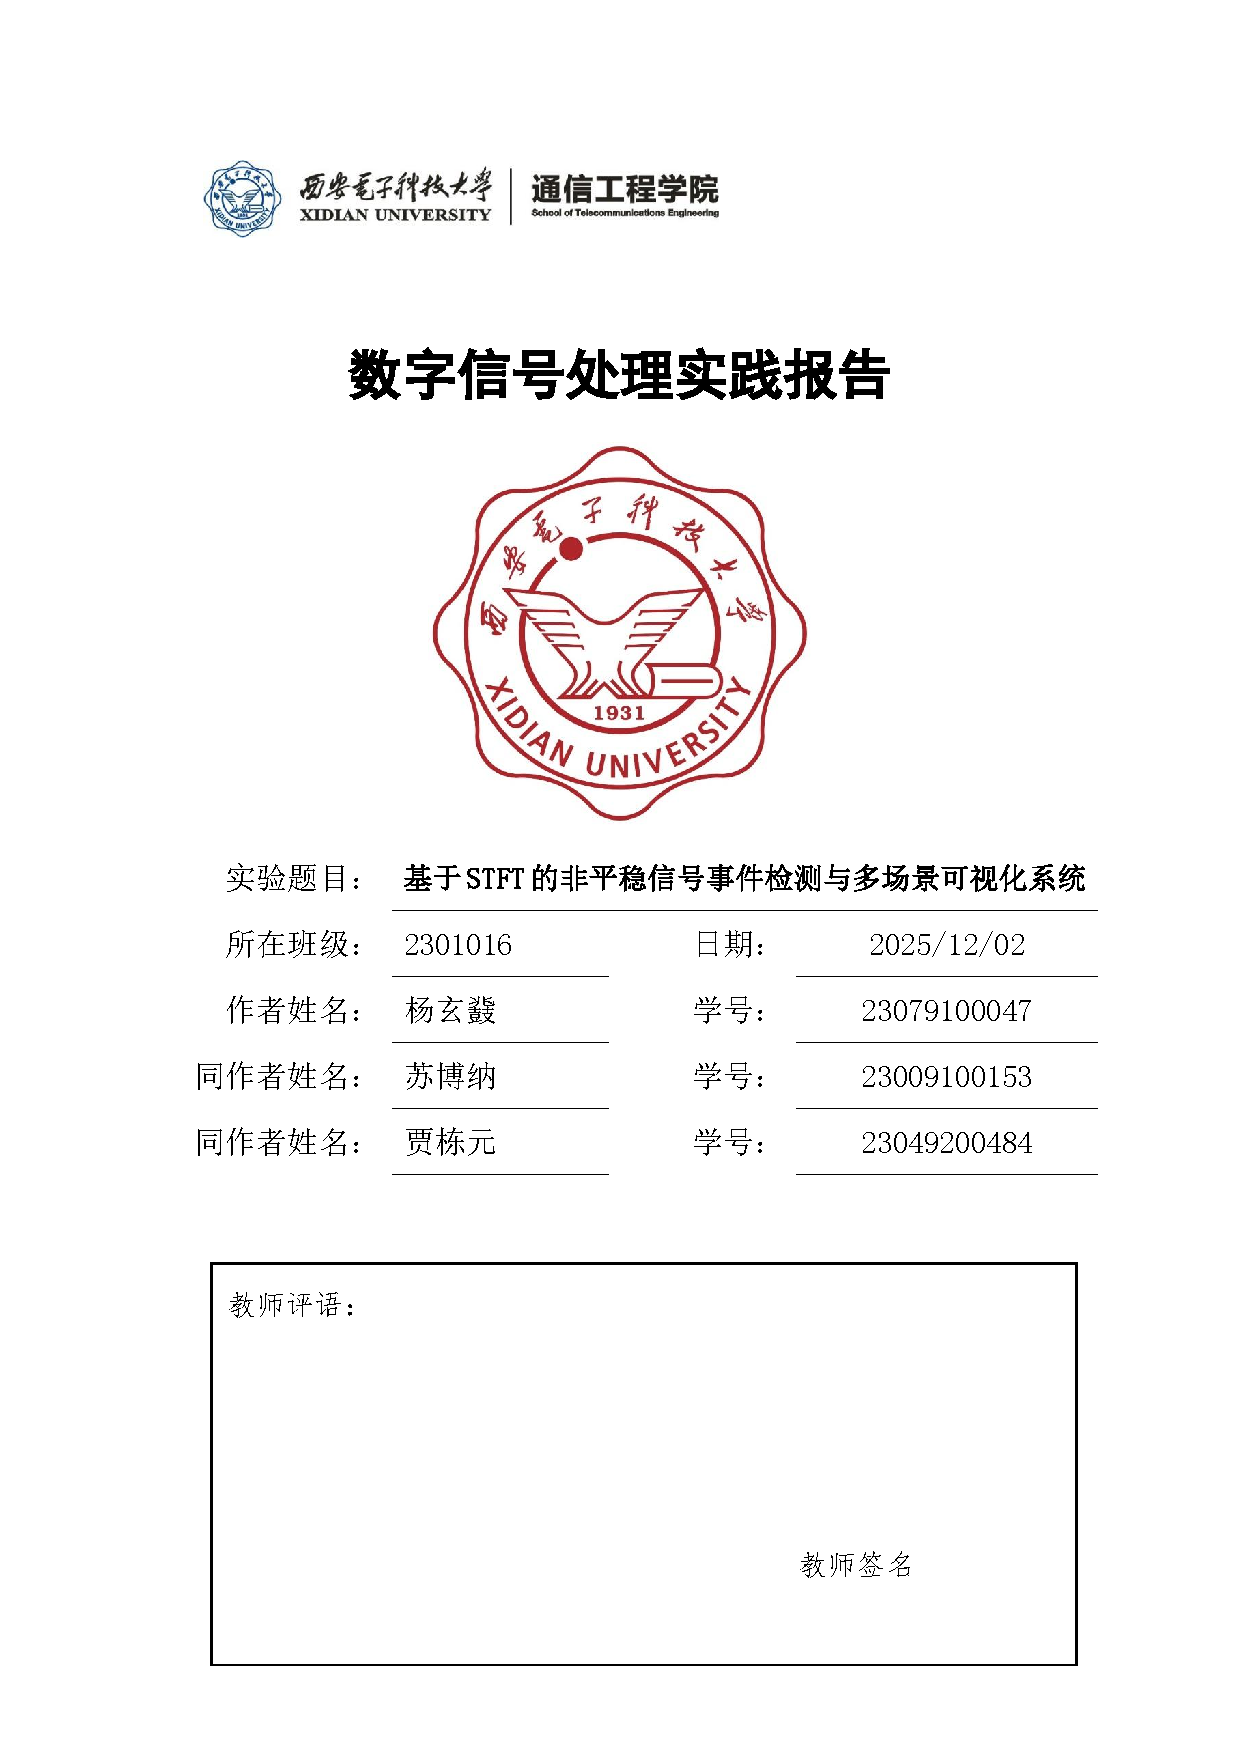
\includepdf[pages=-]{figures/报告封面.pdf}
\end{titlepage}



% ===正文==============================


% 标题（一级居中）

\chapterinline{选题： 基于短时傅里叶变换的非平稳信号事件检测与多场景可视化系统}

\section{研究背景}

在实际工程中，机械振动信号、音乐节奏、语音爆破音、车辆经过产生的多普勒信号等，都属于典型的非平稳信号（Non-stationary Signals）。此类信号的统计特性随时间变化，往往伴随突发冲击、频率跳变、能量瞬变等事件。传统的时域分析方法虽然能够观察到幅度随时间的变化，但难以准确刻画这些事件在频率上的特征，更无法判断事件发生的时间–频率结构。

在 DSP 中，对非平稳信号进行分析的核心工具是短时傅里叶变换（Short-Time Fourier Transform, STFT）。STFT 利用时间窗函数对信号进行分段，能同时揭示信号随时间变化的频谱构成，从而反映事件发生时在频率、能量上的突变。因此，STFT 已成为机械故障诊断、语音分析、音乐处理、雷达与声呐信号处理等领域的重要基础方法。

然而，不同场景下的非平稳事件具有不同的表现形式，例如：

机械冲击信号具有短时高频爆发特性；

鼓点属于瞬时宽带能量突增；

车辆经过带来连续的频率上升–下降（多普勒轨迹）；

语音爆破音则表现为高频能量快速增强；

仅依靠时域难以对这些事件进行统一、准确的分析与检测。

同时，STFT 的分析效果还受到窗函数类型、窗长、重叠率等参数的影响，这些因素直接关系到时间分辨率与频率分辨率之间的平衡。对于初学者或工程人员而言，理解这些参数对非平稳信号分析效果的影响通常较为困难，也缺乏直观的可视化工具帮助理解和实践。

综上，对非平稳信号进行时间–频率联合分析、设计合适的事件检测算法，并构建一个可视化、可调参数的平台，不仅具有重要的理论意义，也具有明确的工程应用价值。

\section{选题目的}

本项目旨在面向典型非平稳信号，构建一个基于短时傅里叶变换的事件检测与可视化分析系统，并实现从信号生成、时频分析、特征提取到事件检测的完整流程。通过本项目希望达到以下目的：

深入理解非平稳信号的时频特征。
通过 STFT、窗函数选择、窗长与重叠率调节等方式直观展示信号的时间–频率变化规律，加深对 DSP 中时频分析理论的掌握。

实现通用的事件检测方法体系。
针对不同事件类型的特征差异，分别从“短时能量突变”“频带能量变化”“谱质心变化”等角度设计事件检测算法，使系统能够适应机械、音乐、语音、车辆等多类非平稳信号。

搭建一个可交互、可视化、可扩展的分析平台。
在 MATLAB App Designer 中构建包含参数滑条、选择控件、自动事件标记和多图并行展示的 UI 界面，使用户能够方便地观察不同参数对分析效果的影响，实现教学、实验与工程实践的一体化。

为多场景下的非平稳事件检测提供统一框架。
系统支持机械振动、音乐节奏信号、车辆多普勒信号等典型场景，为多种现实任务提供事件定位与特征分析能力，具有一定的应用推广价值。

通过本课题的实现，能够系统性展示 DSP 中非平稳信号处理的核心内容，同时使学生在实践中掌握时频分析工具的工程价值与实际应用方法，为进一步学习复杂信号处理、语音分析、医学工程或雷达信号处理奠定基础。

\section{实验内容与方案设计}
\subsection{实验一：典型非平稳信号及其时域观察}

在本实验中，构造了三类具有代表性的非平稳信号：
机械振动冲击信号、音乐鼓点信号以及车辆多普勒信号。
每种信号均包含若干突发事件，其性质分别为：
机械冲击的短时衰减震荡、鼓点的宽带能量瞬态、
以及车辆经过时的连续频率漂移。

实验过程中首先生成三类信号的时域波形，并根据构造时设定的事件位置，
在时域图中标注真实事件时刻。结果表明，不同信号的突发事件在时域上的可见性不尽相同：
机械和音乐事件在时域中具有明显能量突变，而多普勒事件主要体现为频率缓变，
其在时域中的表现并不显著。该现象为后续的时频分析提供了对照依据，
也说明仅依靠时域难以准确识别事件性质。

\subsection{实验二：STFT 时频分析与窗参数影响}

\subsection{实验二：STFT 时频分析与窗参数影响}

本实验针对机械冲击信号，分析不同窗函数与不同窗长对短时频谱的影响。
首先固定窗长为 512，分别采用矩形窗、Hamming 窗、
Hann 窗以及 Blackman 窗进行 STFT 计算。
实验结果显示：矩形窗具有最明显的频谱泄漏现象，旁瓣电平较高；
Hamming 与 Hann 窗有效抑制旁瓣；
而 Blackman 窗旁瓣最低，但主瓣较宽，时间分辨率有所降低。

随后固定窗函数为 Hamming 窗，分别采用不同窗长（128/256/512/1024）进行对比。
实验结果表明：较短的窗（如 128 点）具有较好的时间分辨率，
能够较准确定位冲击事件发生的时刻，但频率分辨率较差；
较长的窗（如 1024 点）具有较高的频率分辨率，
能够更清晰地呈现冲击事件的频率成分，但在时间轴上出现模糊。
该实验直观展示了短时傅里叶变换中时间—频率分辨率的基本权衡关系。


\subsection{实验三：特征提取实验}
\subsection{实验四：事件检测算法设计与参数分析}
\subsection{实验五：多场景非平稳信号的事件检测对比}
\subsection{实验六：检测性能与鲁棒性评估（可选）}


\end{document}